% Diagram wiring UART Raspberry Pi, modul XY-017 (MAX3485), dan bus RS485.
\begin{figure}[H]
\centering
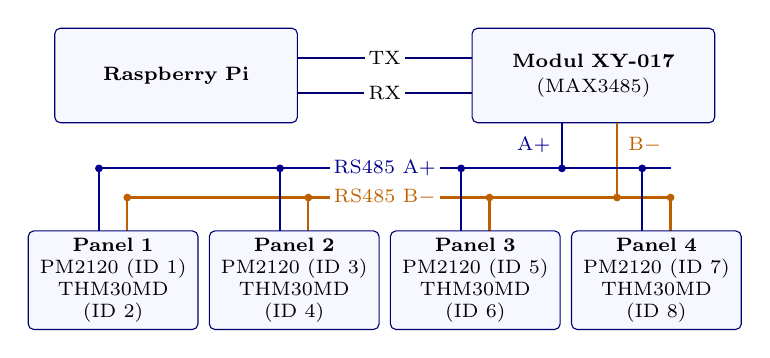
\begin{tikzpicture}[
 font=\rmfamily\fontsize{7.5}{9}\selectfont,
 unit/.style={draw=blue!45!black,rounded corners=2pt,align=center,
 fill=blue!3,inner sep=4pt,text width=2.8cm,minimum height=1.2cm},
 panel/.style={draw=blue!45!black,rounded corners=2pt,align=center,
 fill=blue!3,inner sep=2.5pt,text width=1.98cm,
 font=\rmfamily\fontsize{6.6}{8}\selectfont},
 busa/.style={thick,draw=blue!55!black},
 busb/.style={thick,draw=orange!75!black},
 pinlbl/.style={font=\rmfamily\fontsize{6.8}{8}\selectfont}]

% -- Unit utama: Raspberry Pi dan Modul XY-017 --
\node[unit] (rpi) at (-2.65,0) {\textbf{Raspberry Pi}};
\node[unit] (xy) at (2.65,0) {\textbf{Modul XY-017}\\(MAX3485)};

% -- Jalur RX dan TX antara Raspberry Pi dan Modul XY-017 --
\draw[thick,blue!45!black] (-1.11,0.22) -- (1.11,0.22);
\node[fill=white,inner sep=1.5pt,pinlbl] at (0,0.22) {TX};
\draw[thick,blue!45!black] (-1.11,-0.22) -- (1.11,-0.22);
\node[fill=white,inner sep=1.5pt,pinlbl] at (0,-0.22) {RX};

% -- Keluaran RS485 (A+ dan B-) dari XY-017 ke Bus RS485 --
\draw[busa] (2.25,-0.60) -- (2.25,-1.18);
\node[left,pinlbl,text=blue!55!black] at (2.23,-0.88) {A+};
\draw[busb] (2.95,-0.60) -- (2.95,-1.55);
\node[right,pinlbl,text=orange!75!black] at (2.97,-0.88) {B$-$};

% -- Bus RS485 paralel menuju 4 panel --
\draw[busa] (-3.63,-1.18) -- (3.63,-1.18);
\draw[busb] (-3.27,-1.55) -- (3.63,-1.55);
\fill[blue!55!black] (2.25,-1.18) circle (1.4pt);
\fill[orange!75!black] (2.95,-1.55) circle (1.4pt);
\node[fill=white,inner sep=1.5pt,pinlbl,text=blue!55!black] at (0,-1.18)
 {RS485 A+};
\node[fill=white,inner sep=1.5pt,pinlbl,text=orange!75!black] at (0,-1.55)
 {RS485 B$-$};

% -- Empat panel pada Power Room --
\foreach \x/\pnum/\idm/\idt in {
 -3.45/1/1/2,
 -1.15/2/3/4,
  1.15/3/5/6,
  3.45/4/7/8}{
 \draw[busa] (\x-0.18,-1.18) -- (\x-0.18,-2.10);
 \draw[busb] (\x+0.18,-1.55) -- (\x+0.18,-2.10);
 \fill[blue!55!black] (\x-0.18,-1.18) circle (1.4pt);
 \fill[orange!75!black] (\x+0.18,-1.55) circle (1.4pt);
 \node[panel] at (\x,-2.60)
  {\textbf{Panel \pnum}\\PM2120 (ID \idm)\\THM30MD (ID \idt)};
}
\end{tikzpicture}
\caption{Wiring modul MAX3485 pada node monitoring panel}
\label{fig:panel-uart}
\end{figure}
